% Provenance (never printed): cycle 4 SVT, "La planete Terre": volcanic
% activity, its products and its link with plate boundaries; natural hazards
% and their monitoring; see sources/book1/PROVENANCE.md. Book 1, grade 7,
% chapter 2.
% Vocabulary guard: "magma" first allowed here; "sediment" not before g7.4;
% "subduction zone" is never a term here (gloss: "where one plate sinks under
% another"); "hotspot track" is Book 2's; lahars are called mudflows.
\chapter{Los volcanes}\label{ch:g7:volcanoes}

El 17~de mayo de 1980, un geólogo se situó en una loma a diez kilómetros
del monte Santa Helena, en el noroeste de los Estados Unidos, y tomó la
fotografía de abajo a la izquierda: un cono liso y nevado, una de las
\omterm{def:g1:landscapes-around-us:landform}{montañas} más elegantes del país. Desde hacía dos meses la \omterm{def:g1:landscapes-around-us:landform}{montaña} temblaba,
y su ladera norte se había ido hinchando hacia fuera como un globo. A la
mañana siguiente, a las 8:32, un pequeño \omterm{def:g4:volcanoes-earthquakes-first-look:earthquake}{terremoto} la sacudió. Toda la
ladera hinchada se deslizó, y el \omterm{def:g4:volcanoes-earthquakes-first-look:volcano}{volcán} explotó de lado. Cuando se pudo
volver a fotografiar desde la misma loma, en septiembre, la \omterm{def:g1:landscapes-around-us:landform}{montaña} tenía el
aspecto de la fotografía de la derecha.

\begin{omfigure}
\begin{minipage}[b]{0.495\linewidth}\centering
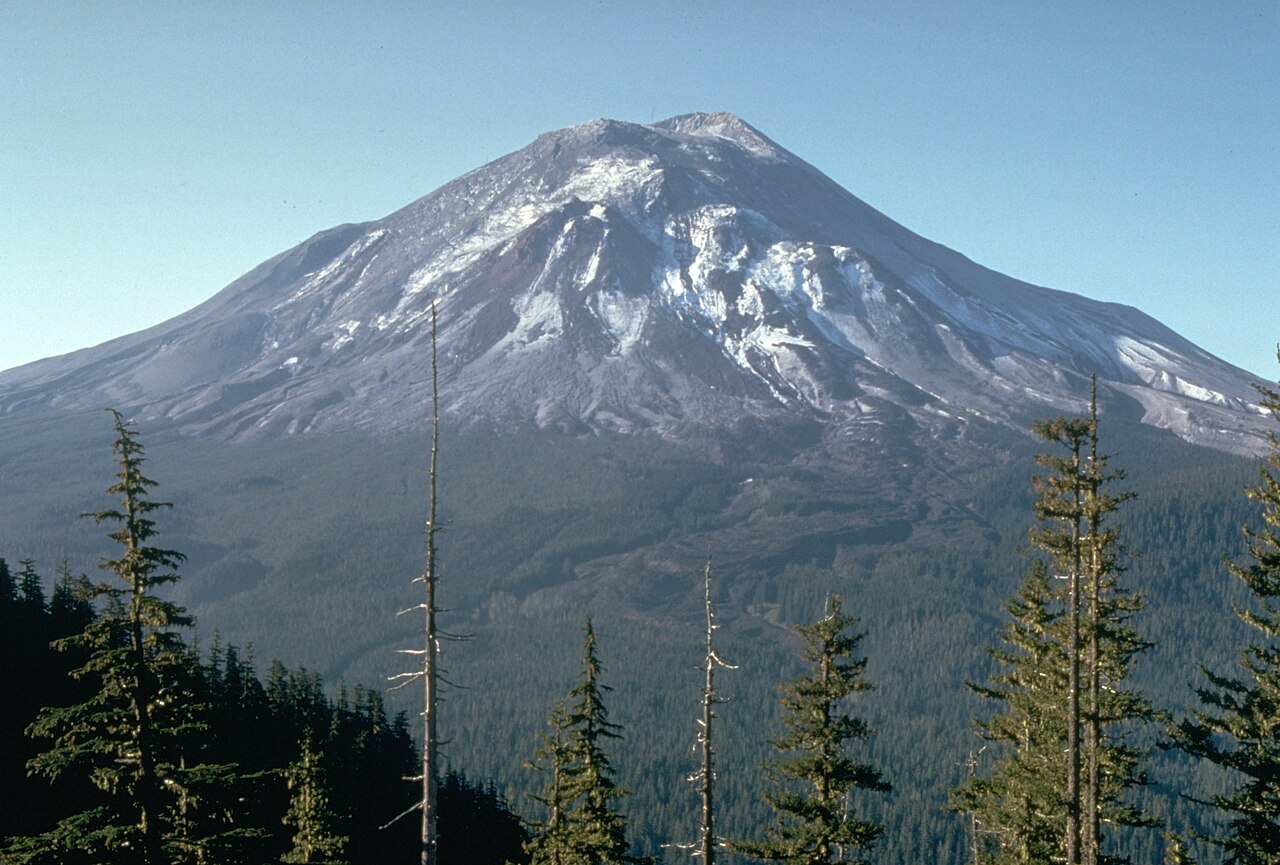
\includegraphics[width=\linewidth]{images/book1/g7-msh-before.jpg}

{\small 17 de mayo de 1980, la víspera.}
\end{minipage}\hfill
\begin{minipage}[b]{0.495\linewidth}\centering
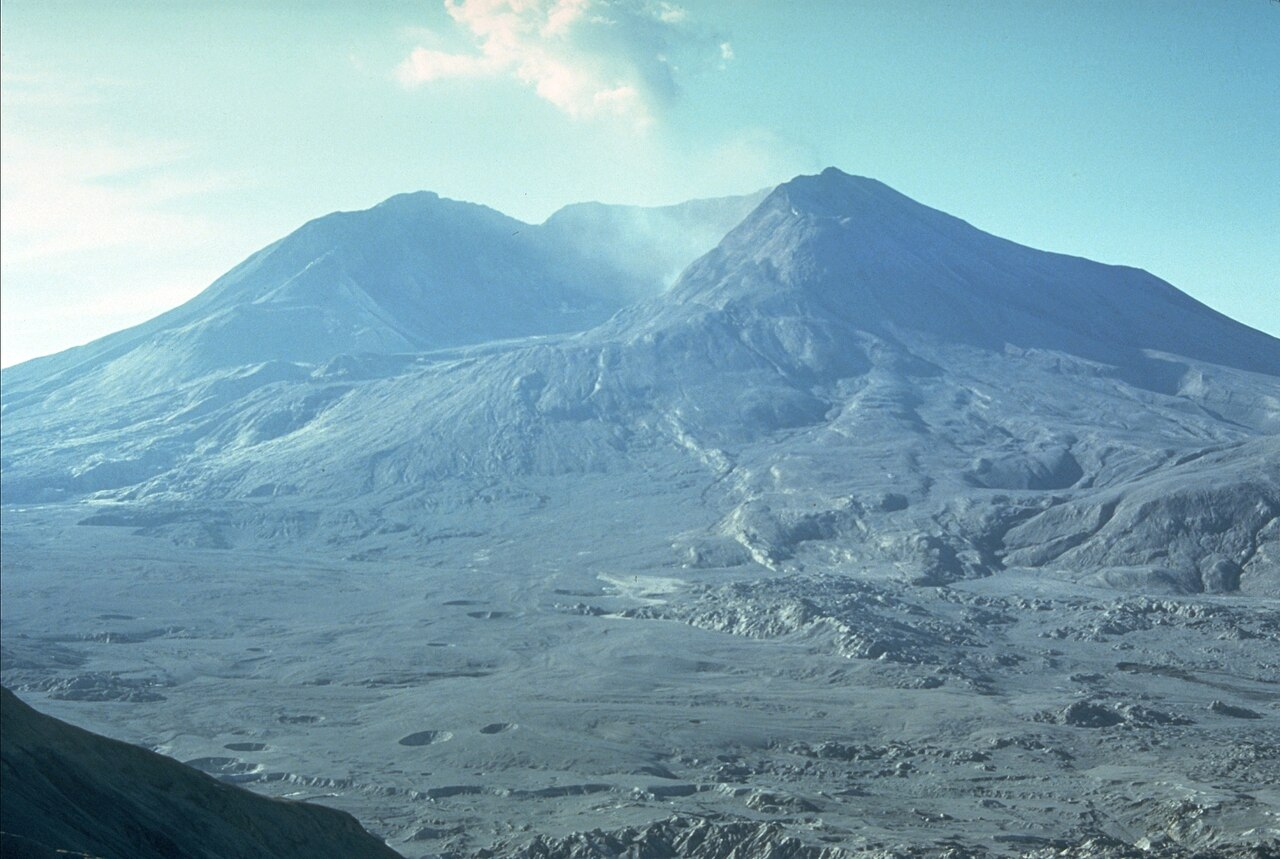
\includegraphics[width=\linewidth]{images/book1/g7-msh-after.jpg}

{\small 10 de septiembre de 1980.}
\end{minipage}

{\small El monte Santa Helena visto desde Johnston Ridge, antes y después de
la \omterm{def:g4:volcanoes-earthquakes-first-look:eruption}{erupción} del 18~de mayo de 1980. La cima y toda la ladera norte han
desaparecido; en su lugar hay un \omterm{def:g7:volcanoes:vent}{cráter} abierto hacia el norte.
Fotografías: Harry Glicken, U.S. Geological Survey (dominio público, vía
Wikimedia Commons).}
% ledger: commons:msh-before, commons:msh-after, usgs:msh-lead-up, usgs:msh-may18
\label{fig:g7:volcanoes:st-helens}
\end{omfigure}

En este capítulo abrimos un \omterm{def:g4:volcanoes-earthquakes-first-look:volcano}{volcán} para ver qué impulsa una \omterm{def:g4:volcanoes-earthquakes-first-look:eruption}{erupción};
averiguamos por qué algunos \omterm{def:g4:volcanoes-earthquakes-first-look:volcano}{volcanes} derraman tranquilos \omterm{def:g1:landscapes-around-us:water}{ríos} de \omterm{def:g4:volcanoes-earthquakes-first-look:eruption}{lava}
mientras otros saltan por los aires; y volvemos a mirar el \omterm{def:g3:continents-and-oceans:world-map}{mapamundi} para
ver dónde están los \omterm{def:g4:volcanoes-earthquakes-first-look:volcano}{volcanes} y por qué.

\begin{recall}
Un \emph{\omterm{def:g4:volcanoes-earthquakes-first-look:volcano}{volcán}} es un lugar donde la \omterm{def:g3:stones-pebbles-sand:rock}{roca} fundida del interior de la Tierra
sale a la superficie, y la \omterm{def:g1:landscapes-around-us:landform}{colina} o la \omterm{def:g1:landscapes-around-us:landform}{montaña} que construye allí. Durante
una \emph{\omterm{def:g4:volcanoes-earthquakes-first-look:eruption}{erupción}}, expulsa \omterm{def:g4:volcanoes-earthquakes-first-look:eruption}{lava}, ceniza y gases
(\cref{ch:g4:volcanoes-earthquakes-first-look}). Bajo la \omterm{def:g6:inside-the-earth:layers}{corteza}, el \omterm{def:g6:inside-the-earth:layers}{manto}
está hecho de \omterm{def:g3:stones-pebbles-sand:rock}{roca} caliente que es sólida, aunque puede deslizarse muy
despacio (\cref{ch:g6:inside-the-earth}). El basalto y el granito son \omterm{def:g6:rocks-and-minerals:rock-families}{rocas
ígneas}: se forman cuando la \omterm{def:g3:stones-pebbles-sand:rock}{roca} fundida se enfría y se endurece
(\cref{ch:g6:rocks-and-minerals}). La envoltura exterior de la Tierra está
rota en \omterm{def:g7:plate-tectonics:plate}{placas} que se desplazan unos pocos centímetros al año; sus bordes
son los \omterm{def:g7:plate-tectonics:plate-boundary}{límites de placas} (\cref{ch:g7:plate-tectonics}).
\end{recall}

\section{El interior de un volcán}

El \omterm{def:g6:inside-the-earth:layers}{manto} es sólido. Sin embargo, en algunos lugares, en las profundidades,
se funde una pequeña parte de la \omterm{def:g3:stones-pebbles-sand:rock}{roca}. La \omterm{def:g3:stones-pebbles-sand:rock}{roca} fundida es más ligera que la
\omterm{def:g3:stones-pebbles-sand:rock}{roca} sólida que la rodea, así que sube despacio, abriéndose paso por las
grietas, como una gota de aceite que sube a través del agua.
% ledger: usgs:hawaii-hotspot (magma lighter than the surrounding rock, rises)

\begin{definition}[Magma]\label{def:g7:volcanoes:magma}
El \emph{magma}\index{magma} es la \omterm{def:g3:stones-pebbles-sand:rock}{roca} fundida que está bajo tierra. Es un
líquido caliente que también puede llevar cristales y, disueltos en él,
gases como el vapor de agua y el dióxido de carbono. El magma que sale a la
superficie se llama \omterm{def:g4:volcanoes-earthquakes-first-look:eruption}{lava}; al salir, pierde la mayor parte de su gas.
\end{definition}

El \omterm{def:g7:volcanoes:magma}{magma} que sube a menudo se detiene por el camino, unos pocos kilómetros
por debajo de la superficie, donde se acumula en una gran bolsa. Allí
espera, a veces durante siglos, antes de que una \omterm{def:g4:volcanoes-earthquakes-first-look:eruption}{erupción} vacíe una parte.

\begin{definition}[Cámara magmática]\label{def:g7:volcanoes:magma-chamber}
Una \emph{cámara magmática}\index{camara magmatica@cámara magmática} es un
gran espacio en las \omterm{def:g3:stones-pebbles-sand:rock}{rocas} que hay bajo un \omterm{def:g4:volcanoes-earthquakes-first-look:volcano}{volcán}, a unos pocos kilómetros
de profundidad, donde se acumula el \omterm{def:g7:volcanoes:magma}{magma} antes de una \omterm{def:g4:volcanoes-earthquakes-first-look:eruption}{erupción}.
\end{definition}

\begin{definition}[Boca eruptiva y cráter]\label{def:g7:volcanoes:vent}
Una \emph{boca eruptiva}\index{boca eruptiva} es una abertura en la
superficie por la que salen el \omterm{def:g7:volcanoes:magma}{magma}, los gases y la ceniza. Un
\emph{cráter}\index{crater@cráter} es la depresión en forma de cuenco que
rodea una boca, normalmente en lo alto del \omterm{def:g4:volcanoes-earthquakes-first-look:volcano}{volcán}.
\end{definition}

\begin{omfigure}
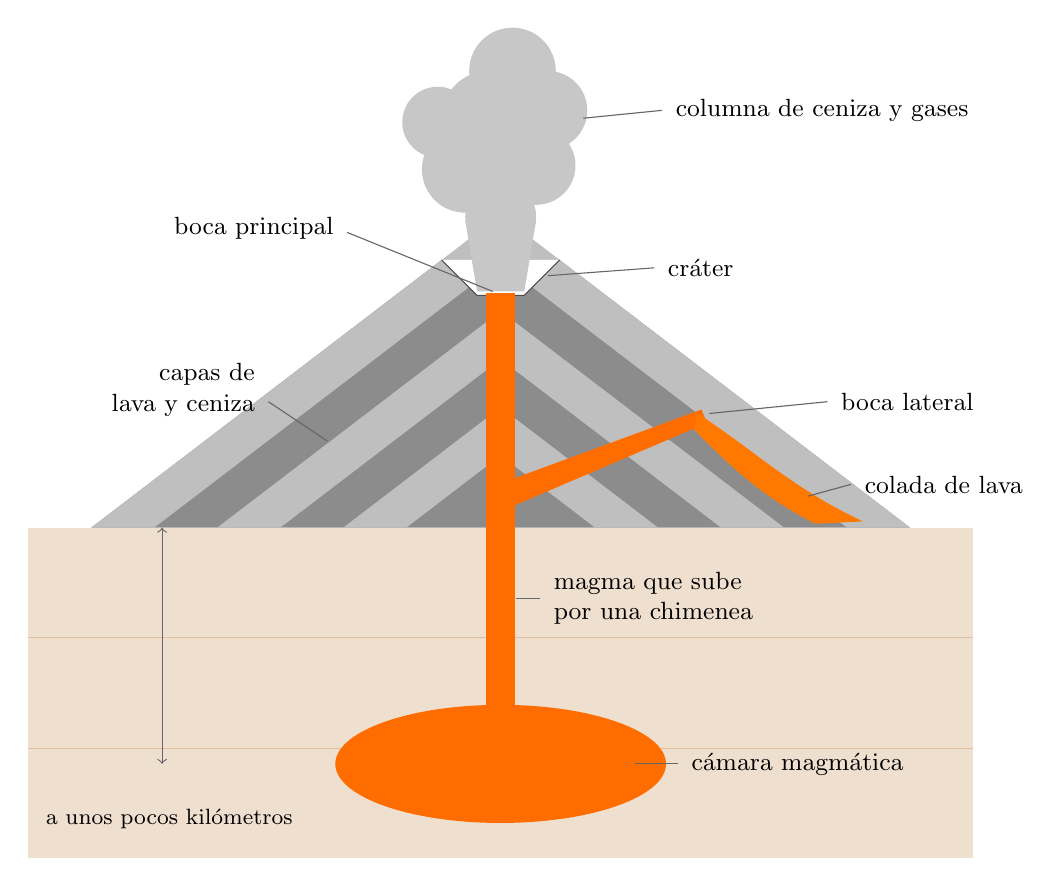
\begin{tikzpicture}[font=\small, x=1cm, y=1cm]
  % rocks below the volcano
  \fill[brown!25] (-6,-4.2) rectangle (6,0);
  \draw[brown!50] (-6,-1.4) -- (6,-1.4) (-6,-2.8) -- (6,-2.8);
  % the cone, built of layers of lava (dark) and ash (light)
  \fill[black!45] (-5.2,0) -- (-0.75,3.4) -- (0.75,3.4) -- (5.2,0) -- cycle;
    % layers dipping outwards, parallel to the flanks (slope 3.4/4.45)
  \foreach \k/\c in {0/black!25, 2/black!25, 4/black!25} {
    \pgfmathsetmacro{\xa}{-5.2+0.8*\k}\pgfmathsetmacro{\xb}{-5.2+0.8*(\k+1)}
    \pgfmathsetmacro{\ya}{(-0.18-\xa)*3.4/4.45}\pgfmathsetmacro{\yb}{(-0.18-\xb)*3.4/4.45}
    \fill[\c] (\xa,0) -- (-0.18,\ya) -- (-0.18,\yb) -- (\xb,0) -- cycle;
    \fill[\c] (-\xa,0) -- (0.18,\ya) -- (0.18,\yb) -- (-\xb,0) -- cycle;
  }
  % the crater at the top
  \fill[white] (-0.75,3.4) -- (-0.3,2.95) -- (0.3,2.95) -- (0.75,3.4) -- cycle;
  \draw[black!70] (-0.75,3.4) -- (-0.3,2.95) -- (0.3,2.95) -- (0.75,3.4);
  % magma chamber and the pipe up to the vent
  \fill[orange!85!red] (0,-3.0) ellipse (2.1 and 0.75);
  \fill[orange!85!red] (-0.18,-2.4) rectangle (0.18,2.98);
  % a side branch to a small side vent
  \fill[orange!85!red] (0.1,0.6) -- (2.55,1.5) -- (2.62,1.33) -- (0.1,0.25) -- cycle;
  % lava flow down the right flank, from the side vent
  \fill[orange!95!red] (2.5,1.45) .. controls (3.2,1.0) and (3.7,0.5) .. (4.6,0.08)
    -- (4.0,0.05) .. controls (3.3,0.4) and (2.9,0.8) .. (2.45,1.25) -- cycle;
  % ash column and gas
    \fill[black!22] (-0.3,3.0) -- (0.3,3.0) -- (0.45,3.9) -- (-0.45,3.9) -- cycle;
  \foreach \x/\y/\r in {0/3.95/0.45, -0.45/4.55/0.55, 0.45/4.6/0.5, -0.15/5.2/0.6,
                        0.6/5.3/0.5, -0.8/5.15/0.45, 0.15/5.8/0.55}
    \fill[black!22] (\x,\y) circle (\r);
  % labels
  \node[anchor=west] at (2.1,5.3) {columna de ceniza y gases};
  \draw[black!60] (2.05,5.3) -- (1.05,5.2);
  \node[anchor=west] at (2.0,3.3) {cráter};
  \draw[black!60] (1.95,3.3) -- (0.6,3.2);
  \node[anchor=east] at (-2.0,3.8) {boca principal};
  \draw[black!60] (-1.95,3.75) -- (-0.1,3.0);
  \node[anchor=west] at (4.2,1.6) {boca lateral};
  \draw[black!60] (4.15,1.6) -- (2.65,1.45);
  \node[anchor=west] at (4.5,0.55) {colada de lava};
  \draw[black!60] (4.45,0.55) -- (3.9,0.4);
  \node[anchor=east, align=right] at (-3.0,1.75) {capas de\\lava y ceniza};
  \draw[black!60] (-2.95,1.6) -- (-2.2,1.1);
  \node[anchor=west, align=left] at (0.55,-0.9) {magma que sube\\por una chimenea};
  \draw[black!60] (0.5,-0.9) -- (0.2,-0.9);
  \node[anchor=west] at (2.3,-3.0) {cámara magmática};
  \draw[black!60] (2.25,-3.0) -- (1.7,-3.0);
  \node[anchor=west, align=left, font=\footnotesize] at (-5.9,-3.7) {a unos pocos kilómetros};
  \draw[black!60, <->] (-4.3,0) -- (-4.3,-3.0);
\end{tikzpicture}

{\small Un \omterm{def:g4:volcanoes-earthquakes-first-look:volcano}{volcán} abierto en canal (un dibujo, no a escala). El \omterm{def:g7:volcanoes:magma}{magma} se
acumula en la \omterm{def:g7:volcanoes:magma-chamber}{cámara magmática} y sube por una chimenea hasta la \omterm{def:g7:volcanoes:vent}{boca}
principal, en el fondo del \omterm{def:g7:volcanoes:vent}{cráter}; una rama llega hasta una \omterm{def:g7:volcanoes:vent}{boca} lateral en
la ladera. Cada \omterm{def:g4:volcanoes-earthquakes-first-look:eruption}{erupción} añade al cono una capa de \omterm{def:g4:volcanoes-earthquakes-first-look:eruption}{lava} o de ceniza.}
\label{fig:g7:volcanoes:cutaway}
\end{omfigure}

Así que la misma \omterm{def:g3:stones-pebbles-sand:rock}{roca} fundida tiene dos nombres. Bajo tierra es
\emph{\omterm{def:g7:volcanoes:magma}{magma}}; una vez que ha salido por una \omterm{def:g7:volcanoes:vent}{boca}, es \emph{\omterm{def:g4:volcanoes-earthquakes-first-look:eruption}{lava}}. La
diferencia no es solo una cuestión de palabras: el \omterm{def:g7:volcanoes:magma}{magma} aún conserva su
gas, mientras que la \omterm{def:g4:volcanoes-earthquakes-first-look:eruption}{lava} ha perdido casi todo el suyo en el aire. Veremos
que ese gas decide qué clase de \omterm{def:g4:volcanoes-earthquakes-first-look:eruption}{erupción} tiene un \omterm{def:g4:volcanoes-earthquakes-first-look:volcano}{volcán}.

¿Cuánto calor hace? Los científicos del Observatorio Vulcanológico de Hawái
miden la \omterm{def:g4:volcanoes-earthquakes-first-look:eruption}{lava} cuando sale por las \omterm{def:g7:volcanoes:vent}{bocas} del Kilauea, uno de los \omterm{def:g4:volcanoes-earthquakes-first-look:volcano}{volcanes} de
Hawái: unos \qty{1170}{\degreeCelsius}. La \omterm{def:g3:stones-pebbles-sand:rock}{roca} caliente brilla, y el color
de ese brillo depende de su temperatura: unas cámaras especiales leen desde
lejos la temperatura de una colada midiendo los colores de su brillo.
Incluso el ojo se hace una idea aproximada, como muestra la tabla.
% ledger: usgs:kilauea-temp, usgs:pyrometer

\begin{center}
\small
\begin{tabular}{|l|c|}
\hline
\textbf{color de la \omterm{def:g3:stones-pebbles-sand:rock}{roca} incandescente} & \textbf{temperatura} \\
\hline
amarillo & de unos 1000 a \qty{1200}{\degreeCelsius} \\
naranja & de unos 800 a \qty{1000}{\degreeCelsius} \\
rojo & de unos 600 a \qty{800}{\degreeCelsius} \\
\hline
\end{tabular}
\end{center}
% ledger: usgs:kilauea-temp

\begin{remark}[Una piel que se enfría en un segundo]\label{rem:g7:volcanoes:skin}
% ledger: usgs:kilauea-temp
Cuando la \omterm{def:g4:volcanoes-earthquakes-first-look:eruption}{lava} toca el aire por primera vez, su superficie se enfría
cientos de grados cada segundo: enseguida se forma una piel oscura sobre la
\omterm{def:g3:stones-pebbles-sand:rock}{roca} incandescente. Bajo la piel, la \omterm{def:g4:volcanoes-earthquakes-first-look:eruption}{lava} sigue caliente mucho tiempo. En
Hawái, la \omterm{def:g4:volcanoes-earthquakes-first-look:eruption}{lava} ha corrido por túneles bajo su propio techo endurecido a lo
largo de \qty{10}{km}, desde una \omterm{def:g7:volcanoes:vent}{boca} hasta el \omterm{def:g2:water-on-earth:ocean}{mar}, y aun así ha llegado a
la orilla a unos \qty{1140}{\degreeCelsius}: solo unos 30~grados menos que
en la \omterm{def:g7:volcanoes:vent}{boca}.
\end{remark}

\begin{omfigure}
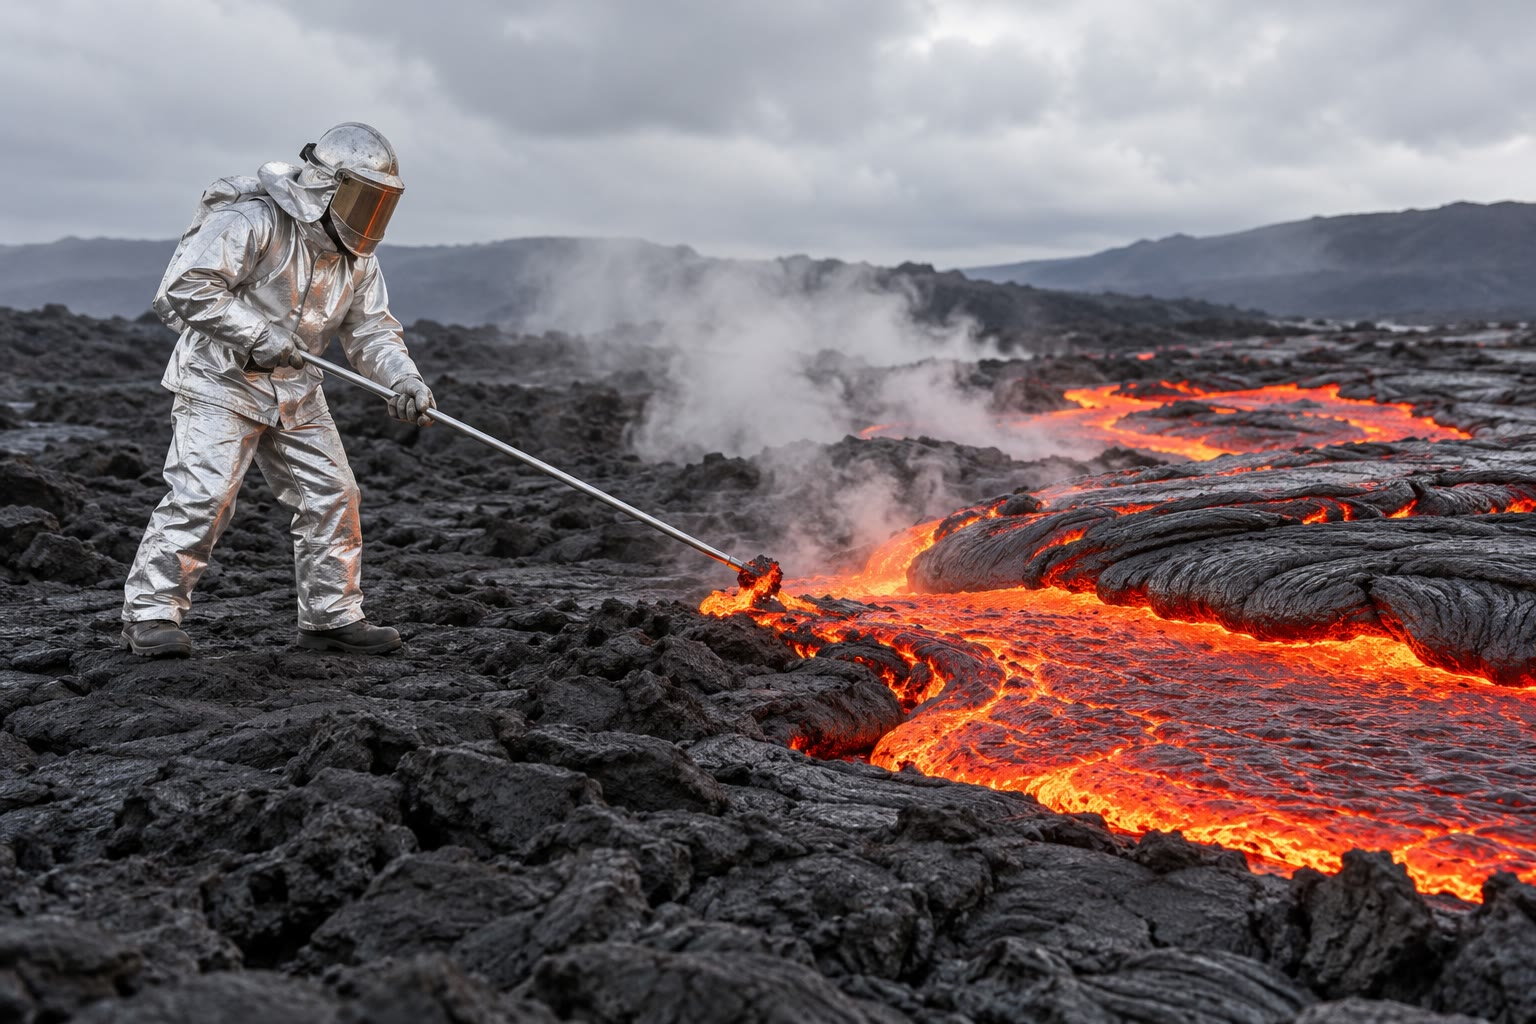
\includegraphics[width=0.6\linewidth]{images/book1/ai/g7-volcanologist.jpg}

{\small Una vulcanóloga con un traje que refleja el calor toma una muestra
de \omterm{def:g4:volcanoes-earthquakes-first-look:eruption}{lava} con una larga barra de acero (ilustración generada por IA de una
escena genérica). Solo los científicos formados, con este tipo de equipo, se
acercan a la \omterm{def:g4:volcanoes-earthquakes-first-look:eruption}{lava} que corre; todos los demás miran desde donde lo permiten
las autoridades.}
\label{fig:g7:volcanoes:volcanologist}
\end{omfigure}

\section{Dos maneras de entrar en erupción}

El monte Santa Helena saltó por los aires. Los \omterm{def:g4:volcanoes-earthquakes-first-look:volcano}{volcanes} de Hawái, en
cambio, suelen derramar \omterm{def:g4:volcanoes-earthquakes-first-look:eruption}{lava} que corre por sus laderas. Los geólogos
clasifican las \omterm{def:g4:volcanoes-earthquakes-first-look:eruption}{erupciones} en dos clases.

\begin{definition}[Erupciones efusivas y explosivas]\label{def:g7:volcanoes:eruption-types}
En una \emph{erupción efusiva}\index{erupcion efusiva@erupción efusiva} el
\omterm{def:g7:volcanoes:magma}{magma} sale tranquilamente en forma de \omterm{def:g4:volcanoes-earthquakes-first-look:eruption}{lava}, que se aleja de la \omterm{def:g7:volcanoes:vent}{boca},
a veces a lo largo de kilómetros, o salta en fuentes de gotas
incandescentes. En una \emph{erupción
explosiva}\index{erupcion explosiva@erupción explosiva} el \omterm{def:g7:volcanoes:magma}{magma}
salta en pedazos por la fuerza de su propio gas: una columna de ceniza,
gases y trozos de \omterm{def:g3:stones-pebbles-sand:rock}{roca} sale lanzada muy alto hacia el cielo.
\end{definition}

\begin{omfigure}
\begin{minipage}[t]{0.49\linewidth}\centering
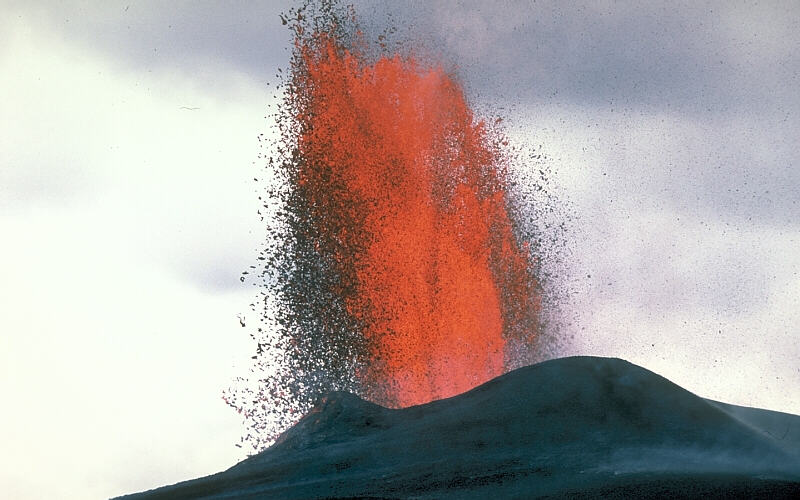
\includegraphics[height=4.5cm]{images/book1/g7-lava-fountain.jpg}

{\small Efusiva: una fuente de \omterm{def:g4:volcanoes-earthquakes-first-look:eruption}{lava} en el Kilauea, Hawái, en 1983.
Fotografía: J.~D. Griggs, USGS.}
\end{minipage}\hfill
\begin{minipage}[t]{0.49\linewidth}\centering
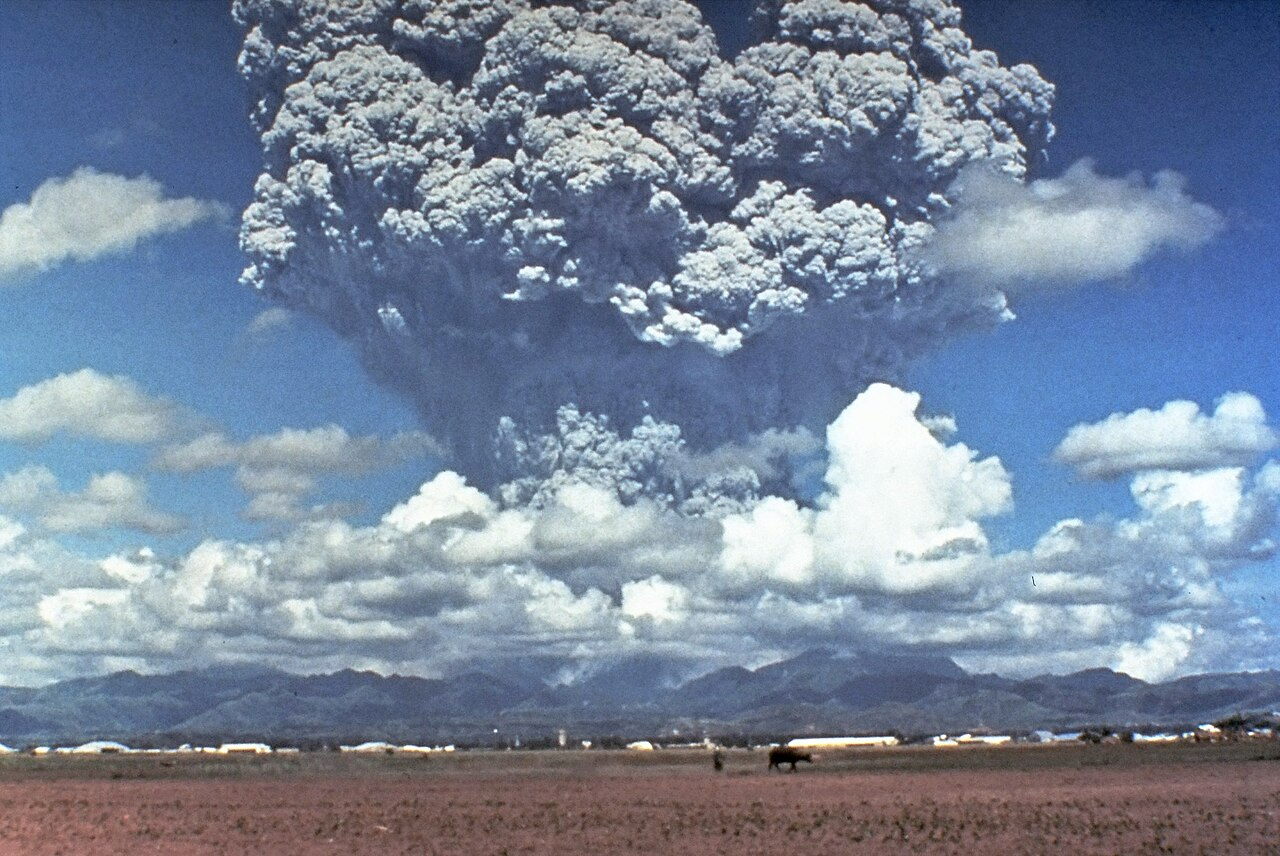
\includegraphics[height=4.5cm]{images/book1/g7-pinatubo.jpg}

{\small Explosiva: la columna eruptiva del monte Pinatubo, Filipinas, el
12~de junio de 1991. Fotografía: Dave Harlow, USGS.}
\end{minipage}\par\medskip


{\small Las dos fotografías son de dominio público (vía Wikimedia
Commons).}
% ledger: commons:lava-fountain, commons:pinatubo
\label{fig:g7:volcanoes:two-photos}
\end{omfigure}

¿Qué marca la diferencia? Dos cosas: lo fluido que es el \omterm{def:g7:volcanoes:magma}{magma} y la
cantidad de gas que contiene.

\textbf{Fluido o viscoso.} Algunos \omterm{def:g7:volcanoes:magma}{magmas} son fluidos, casi como la miel
caliente: es el caso del \omterm{def:g7:volcanoes:magma}{magma} que, al enfriarse, da el basalto oscuro, como
en Hawái. Otros \omterm{def:g7:volcanoes:magma}{magmas} son espesos y viscosos, como la miel fría o la pasta
de dientes. A través de un \omterm{def:g7:volcanoes:magma}{magma} fluido, las burbujas de gas suben
fácilmente y escapan en la superficie, unas pocas cada vez. En un \omterm{def:g7:volcanoes:magma}{magma}
viscoso, las burbujas quedan atrapadas.

\textbf{Poco o mucho gas.} Una botella de agua con gas contiene mucho gas
disuelto en el agua, mantenido allí por la presión del interior de la
botella cerrada; no se ve. Abre la botella y la presión baja: aparecen
burbujas por todas partes, y si se ha agitado la botella, la espuma sale
disparada. El \omterm{def:g7:volcanoes:magma}{magma} de las profundidades también contiene gas disuelto a
alta presión. Al subir, la presión baja y el gas sale de la disolución en
forma de burbujas.
% ledger: usgs:volcanic-gases

Juntemos las dos cosas. Un \omterm{def:g7:volcanoes:magma}{magma} fluido con poco gas deja escapar sus
burbujas y sale en forma de \omterm{def:g4:volcanoes-earthquakes-first-look:eruption}{lava} que corre: la \omterm{def:g4:volcanoes-earthquakes-first-look:eruption}{erupción} es efusiva. Un
\omterm{def:g7:volcanoes:magma}{magma} viscoso lleno de gas retiene sus burbujas hasta que se hinchan tanto
que desgarran el \omterm{def:g7:volcanoes:magma}{magma} en jirones: la \omterm{def:g4:volcanoes-earthquakes-first-look:eruption}{erupción} es explosiva. Los jirones de
\omterm{def:g7:volcanoes:magma}{magma} espumoso se solidifican en el aire en forma de ceniza y de piedra
pómez, una \omterm{def:g3:stones-pebbles-sand:rock}{roca} tan llena de burbujas que puede flotar.

\begin{example}[Pinatubo, 1991: el refresco sin gas y el refresco agitado]\label{ex:g7:volcanoes:pinatubo}
% ledger: usgs:pinatubo-1991
En junio de~1991, el primer \omterm{def:g7:volcanoes:magma}{magma} llegó a la superficie del monte Pinatubo,
en Filipinas. Por el camino había perdido la mayor parte de su gas, ``como
una botella de refresco que se ha quedado sin gas'', en palabras de los
científicos que lo vigilaban. Salió despacio y se amontonó formando un
domo sobre la \omterm{def:g7:volcanoes:vent}{boca}: no hubo explosión. Después, el 12~de junio, un \omterm{def:g7:volcanoes:magma}{magma}
todavía lleno de gas llegó a la superficie y explotó --- la columna de la
fotografía de arriba. El 15~de junio llegó un \omterm{def:g7:volcanoes:magma}{magma} aún más rico en gas, y
el \omterm{def:g4:volcanoes-earthquakes-first-look:volcano}{volcán} tuvo una de las mayores \omterm{def:g4:volcanoes-earthquakes-first-look:eruption}{erupciones} del siglo~XX: expulsó más de
cinco kilómetros cúbicos de \omterm{def:g3:stones-pebbles-sand:rock}{roca} y ceniza, su \omterm{def:g4:clouds-rain-snow:cloud}{nube} de ceniza subió a
\qty{35}{km} de altura, y la cima de la \omterm{def:g1:landscapes-around-us:landform}{montaña} se hundió y dejó una
depresión de \qty{2.5}{km} de diámetro. El mismo \omterm{def:g4:volcanoes-earthquakes-first-look:volcano}{volcán}, la misma semana:
el gas marcó la diferencia.
\end{example}

La forma de un \omterm{def:g4:volcanoes-earthquakes-first-look:volcano}{volcán} guarda la memoria de sus \omterm{def:g4:volcanoes-earthquakes-first-look:eruption}{erupciones}. La \omterm{def:g4:volcanoes-earthquakes-first-look:eruption}{lava} fluida
corre lejos antes de endurecerse, así que, capa tras capa, construye una
\omterm{def:g1:landscapes-around-us:landform}{montaña} ancha de laderas suaves, con la forma de un escudo de guerrero
tendido en el suelo: un \emph{\omterm{def:g4:volcanoes-earthquakes-first-look:volcano}{volcán} en escudo}. El Mauna Loa, en Hawái, es
uno de ellos. La \omterm{def:g4:volcanoes-earthquakes-first-look:eruption}{lava} viscosa y la ceniza se amontonan cerca de la \omterm{def:g7:volcanoes:vent}{boca} y
forman un cono empinado hecho de capas de \omterm{def:g4:volcanoes-earthquakes-first-look:eruption}{lava} y de ceniza: un
\emph{estratovolcán} (\emph{estrato} significa capa). El monte Santa Helena
y el Pinatubo son dos de ellos.

\begin{omfigure}
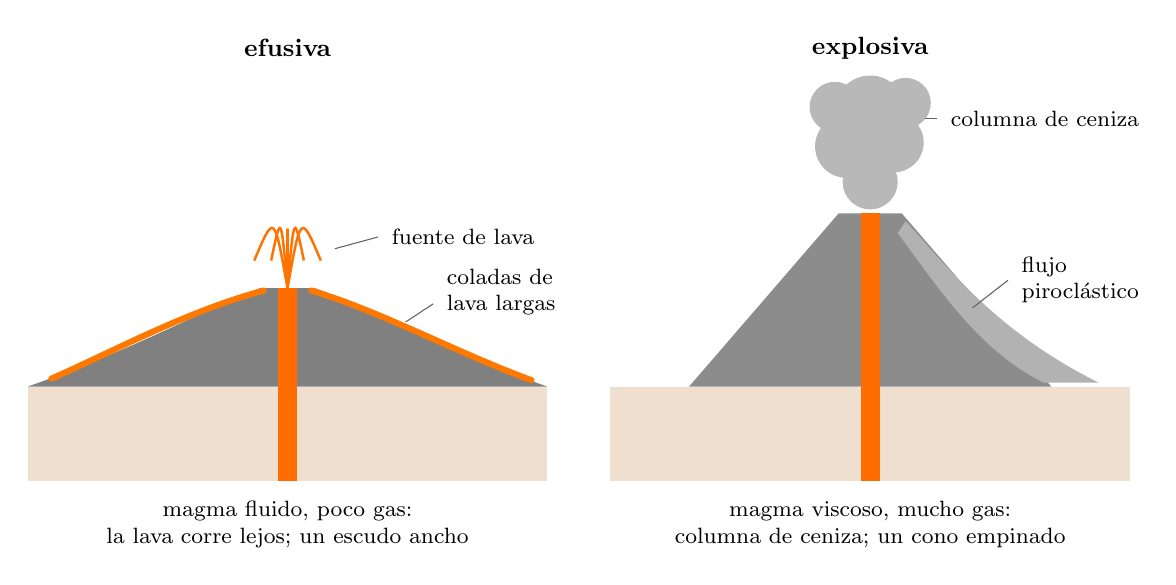
\begin{tikzpicture}[font=\small, x=1cm, y=1cm]
  % --- left: effusive, a shield
  \begin{scope}
    \fill[brown!25] (-3.3,-1.2) rectangle (3.3,0);
    \fill[black!50] (-3.3,0) .. controls (-2.0,0.45) and (-1.0,1.0) .. (-0.35,1.25)
      -- (0.35,1.25) .. controls (1.0,1.0) and (2.0,0.45) .. (3.3,0) -- cycle;
    \fill[orange!85!red] (-0.12,-1.2) rectangle (0.12,1.25);
    % fountain
    \foreach \a in {-25,-12,0,12,25}
      \draw[orange!90!red, line width=0.9pt] (0,1.25) .. controls ({0.4*sin(\a)},2.2) .. ({1.0*sin(\a)},1.6);
    % lava flows far down the gentle slopes
    \draw[orange!95!red, line width=2.2pt, line cap=round] (0.3,1.22) .. controls (1.2,0.95) and (2.1,0.45) .. (3.1,0.08);
    \draw[orange!95!red, line width=2.2pt, line cap=round] (-0.3,1.22) .. controls (-1.3,0.95) and (-2.2,0.45) .. (-3.0,0.1);
    \node[font=\small\bfseries] at (0,4.3) {efusiva};
    \node[align=center, font=\footnotesize] at (0,-1.75) {magma fluido, poco gas:\\la lava corre lejos; un escudo ancho};
    \node[anchor=west, font=\footnotesize] at (1.2,1.9) {fuente de lava};
    \draw[black!60] (1.15,1.9) -- (0.6,1.75);
    \node[anchor=west, font=\footnotesize, align=left] at (1.9,1.2) {coladas de\\lava largas};
    \draw[black!60] (1.85,1.05) -- (1.5,0.82);
  \end{scope}
  % --- right: explosive, a steep cone
  \begin{scope}[xshift=7.4cm]
    \fill[brown!25] (-3.3,-1.2) rectangle (3.3,0);
    \fill[black!45] (-2.3,0) -- (-0.4,2.2) -- (0.4,2.2) -- (2.3,0) -- cycle;
    \fill[orange!85!red] (-0.12,-1.2) rectangle (0.12,2.2);
    \foreach \x/\y/\r in {0/2.6/0.35, -0.3/3.05/0.4, 0.3/3.1/0.38, 0/3.5/0.45, -0.45/3.55/0.32, 0.45/3.6/0.32}
      \fill[black!28] (\x,\y) circle (\r);
    % pyroclastic flow down the flank
    \fill[black!30] (0.45,2.1) .. controls (1.0,1.5) and (1.6,0.7) .. (2.9,0.05)
      -- (2.2,0.05) .. controls (1.4,0.45) and (0.9,1.2) .. (0.35,1.95) -- cycle;
    \node[font=\small\bfseries] at (0,4.3) {explosiva};
    \node[align=center, font=\footnotesize] at (0,-1.75) {magma viscoso, mucho gas:\\columna de ceniza; un cono empinado};
    \node[anchor=west, font=\footnotesize] at (0.9,3.4) {columna de ceniza};
    \draw[black!60] (0.85,3.4) -- (0.7,3.4);
    \node[anchor=west, font=\footnotesize, align=left] at (1.8,1.35) {flujo\\piroclástico};
    \draw[black!60] (1.75,1.35) -- (1.3,1.0);
  \end{scope}
\end{tikzpicture}

{\small Las dos clases de \omterm{def:g4:volcanoes-earthquakes-first-look:eruption}{erupción} y los \omterm{def:g4:volcanoes-earthquakes-first-look:volcano}{volcanes} que construyen (dibujos,
no a escala).}
\label{fig:g7:volcanoes:two-kinds}
\end{omfigure}

\begin{method}[¿Efusiva o explosiva? Cuatro pistas]\label{met:g7:volcanoes:clues}
Para saber, a partir de una descripción o de una fotografía, qué clase de
\omterm{def:g4:volcanoes-earthquakes-first-look:eruption}{erupción} tiene un \omterm{def:g4:volcanoes-earthquakes-first-look:volcano}{volcán}, busca estas pistas.
\begin{enumerate}
  \item \emph{¿Qué sale?} \omterm{def:g4:volcanoes-earthquakes-first-look:eruption}{Lava} que corre o que salta en fuentes: efusiva.
        Una columna de ceniza, trozos de \omterm{def:g3:stones-pebbles-sand:rock}{roca} lanzados: explosiva.
  \item \emph{La forma del \omterm{def:g4:volcanoes-earthquakes-first-look:volcano}{volcán}.} Una \omterm{def:g1:landscapes-around-us:landform}{montaña} ancha de laderas suaves:
        \omterm{def:g4:volcanoes-earthquakes-first-look:eruption}{erupciones} sobre todo efusivas. Un cono empinado: a menudo
        explosivas.
  \item \emph{El \omterm{def:g7:volcanoes:magma}{magma}.} Fluido, poco gas: efusiva. Viscoso, mucho gas:
        explosiva.
  \item \emph{Las \omterm{def:g3:stones-pebbles-sand:rock}{rocas} que quedan.} Coladas de \omterm{def:g4:volcanoes-earthquakes-first-look:eruption}{lava} oscuras y macizas:
        efusiva. Capas de ceniza y de piedra pómez: explosiva.
\end{enumerate}
\end{method}

\begin{example}[Usar las pistas]\label{ex:g7:volcanoes:clues}
Una viajera describe un \omterm{def:g4:volcanoes-earthquakes-first-look:volcano}{volcán}: ``una \omterm{def:g1:landscapes-around-us:landform}{montaña} enorme, suavemente
redondeada, con coladas de \omterm{def:g4:volcanoes-earthquakes-first-look:eruption}{lava} negra por todas sus laderas, algunas de
solo unos pocos años''. La pista~2 (laderas suaves) y la pista~4 (coladas de
\omterm{def:g4:volcanoes-earthquakes-first-look:eruption}{lava} oscuras) apuntan a \omterm{def:g7:volcanoes:eruption-types}{erupciones efusivas}: es un \omterm{def:g4:volcanoes-earthquakes-first-look:volcano}{volcán} en escudo, como el
Mauna Loa.
\end{example}

\begin{inthelab}[Un volcán en una botella (en clase, con el profesor)]
El profesor coge dos botellas cerradas de agua con gas. Una se ha dejado
quieta; la otra se ha agitado suavemente. Las dos se abren al aire libre,
sobre una palangana, apuntando lejos de todo el mundo. La botella quieta
sisea y deja subir unas pocas burbujas; la agitada estalla en una espuma
que sale disparada. ¿Qué botella se parece al \omterm{def:g7:volcanoes:magma}{magma} de Hawái, y cuál al del
Pinatubo? Después, echa un trozo de piedra pómez y un \omterm{def:g3:stones-pebbles-sand:pebble}{canto rodado} en un
cuenco de agua: la piedra pómez flota. Mírala con una lupa: está llena de
agujeros, las burbujas de gas que quedaron congeladas en la \omterm{def:g3:stones-pebbles-sand:rock}{roca} cuando
estalló el \omterm{def:g7:volcanoes:magma}{magma}.
\end{inthelab}

\section{Lo que sale de un volcán}

Una \omterm{def:g4:volcanoes-earthquakes-first-look:eruption}{erupción} expulsa mucho más que \omterm{def:g4:volcanoes-earthquakes-first-look:eruption}{lava}: gases, ceniza, trozos de \omterm{def:g3:stones-pebbles-sand:rock}{roca} y,
en los peores casos, avalanchas de ceniza caliente.

El gas más abundante, con mucho, es el vapor de agua. Las grandes
\omterm{def:g4:volcanoes-earthquakes-first-look:eruption}{erupciones} liberan enormes cantidades de gas en poco tiempo: se calcula que
en un solo día de 1991 el Pinatubo envió más de 250~millones de toneladas de
gas a la alta atmósfera.
% ledger: usgs:volcanic-gases

\begin{definition}[Flujo piroclástico]\label{def:g7:volcanoes:pyroclastic-flow}
Un \emph{flujo piroclástico}\index{flujo piroclastico@flujo piroclástico}
es una avalancha rápida de gas caliente, ceniza y trozos de \omterm{def:g3:stones-pebbles-sand:rock}{roca}, desde
granos de polvo hasta bloques, que baja a toda velocidad por las laderas de
un \omterm{def:g4:volcanoes-earthquakes-first-look:volcano}{volcán} durante una \omterm{def:g7:volcanoes:eruption-types}{erupción explosiva}. (\emph{Piro} significa fuego, y
\emph{clástico}, hecho de trozos rotos.)
\end{definition}

Los \omterm{def:g7:volcanoes:pyroclastic-flow}{flujos piroclásticos} suelen moverse a más de \qty{80}{km/h}, y las \omterm{def:g3:stones-pebbles-sand:rock}{rocas}
y el gas que llevan están en general entre 200 y \qty{700}{\degreeCelsius}.
Por lo general siguen los \omterm{def:g1:landscapes-around-us:landform}{valles}, como el agua, y derriban, queman o
sepultan casi todo lo que encuentran a su paso. El 18~de mayo de 1980, los \omterm{def:g7:volcanoes:pyroclastic-flow}{flujos piroclásticos} del monte
Santa Helena corrieron a entre 80 y \qty{130}{km/h}, a una temperatura de al
menos \qty{700}{\degreeCelsius}, y llegaron a \qty{8}{km} del \omterm{def:g7:volcanoes:vent}{cráter}.
% ledger: usgs:pyroclastic-flows, usgs:msh-flows, usgs:msh-reach

La tabla resume los productos de un \omterm{def:g4:volcanoes-earthquakes-first-look:volcano}{volcán}.

\begin{center}
\small
\begin{tabular}{|p{0.2\linewidth}|p{0.4\linewidth}|p{0.3\linewidth}|}
\hline
\textbf{producto} & \textbf{qué es} & \textbf{el peligro} \\
\hline
colada de \omterm{def:g4:volcanoes-earthquakes-first-look:eruption}{lava} & \omterm{def:g3:stones-pebbles-sand:rock}{roca} fundida que corre por el suelo y después se endurece & quema y sepulta lo que encuentra, pero suele ser lo bastante lenta para que la gente se aparte \\
\hline
ceniza & trocitos diminutos de \omterm{def:g3:stones-pebbles-sand:rock}{roca} y de vidrio, lanzados al aire & cae muy lejos; los tejados se hunden bajo su peso; daña los aviones \\
\hline
bombas volcánicas & trozos de \omterm{def:g4:volcanoes-earthquakes-first-look:eruption}{lava} lanzados que se endurecen mientras vuelan & aplastan lo que golpean, cerca de la \omterm{def:g7:volcanoes:vent}{boca} \\
\hline
gases & sobre todo vapor de agua, después dióxido de carbono y dióxido de azufre & algunos son venenosos; el dióxido de carbono se acumula en las hondonadas \\
\hline
\omterm{def:g7:volcanoes:pyroclastic-flow}{flujo piroclástico} & una avalancha de ceniza, \omterm{def:g3:stones-pebbles-sand:rock}{roca} y gas calientes & el más mortífero: demasiado rápido y demasiado caliente para escapar de él \\
\hline
colada de \omterm{def:g3:stones-pebbles-sand:sand}{barro} & ceniza y \omterm{def:g3:stones-pebbles-sand:rock}{roca} mezcladas con agua de \omterm{def:g4:clouds-rain-snow:precipitation}{lluvia} o de \omterm{def:g4:clouds-rain-snow:precipitation}{nieve} fundida & baja a toda velocidad por los \omterm{def:g1:landscapes-around-us:landform}{valles}, a veces lejos del \omterm{def:g4:volcanoes-earthquakes-first-look:volcano}{volcán} \\
\hline
\end{tabular}
\end{center}
% ledger: usgs:lava-flows, usgs:volcanic-gases, usgs:pyroclastic-flows, usgs:pinatubo-1991, usgs:msh-flows

\begin{method}[¿Cuánto tarda?]\label{met:g7:volcanoes:time}
Para saber cuánto tarda algo que se mueve a una velocidad conocida en
recorrer una distancia, divide la distancia entre la velocidad:
\[
\text{tiempo} = \frac{\text{distancia}}{\text{velocidad}}.
\]
Con una distancia en kilómetros y una velocidad en kilómetros por hora, el
tiempo sale en horas; multiplica por 60 para obtenerlo en minutos.
\end{method}

\begin{example}[Una carrera contra un flujo piroclástico]\label{ex:g7:volcanoes:race}
Un \omterm{def:g7:volcanoes:pyroclastic-flow}{flujo piroclástico} que avanza a \qty{120}{km/h} se dirige hacia un
pueblo situado \qty{6}{km} \omterm{def:g1:landscapes-around-us:landform}{valle} abajo. Tarda $6 \div 120 = 0.05$~horas, es
decir, $0.05 \times 60 = 3$~minutos. Tres minutos: nadie puede salir del
\omterm{def:g1:landscapes-around-us:landform}{valle} a tiempo, ni corriendo ni en coche. La gente solo está a salvo si se
ha marchado \emph{antes} de la \omterm{def:g4:volcanoes-earthquakes-first-look:eruption}{erupción}.
\end{example}

\begin{remark}[Las coladas de barro: el peligro que llega después]\label{rem:g7:volcanoes:mudflows}
% ledger: usgs:msh-flows, usgs:pinatubo-lahars
Una \omterm{def:g4:volcanoes-earthquakes-first-look:eruption}{erupción} deja las laderas cubiertas de ceniza suelta. Cuando le cae la
\omterm{def:g4:clouds-rain-snow:precipitation}{lluvia}, o cuando el calor funde la \omterm{def:g4:clouds-rain-snow:precipitation}{nieve} y el hielo de la cima, la ceniza
se convierte en coladas de \omterm{def:g3:stones-pebbles-sand:sand}{barro} que bajan a toda velocidad por los \omterm{def:g1:landscapes-around-us:landform}{valles}.
El 18~de mayo de 1980, las coladas de \omterm{def:g3:stones-pebbles-sand:sand}{barro} del monte Santa Helena dañaron
27~puentes y casi 200~viviendas. Alrededor del Pinatubo, las fuertes
\omterm{def:g4:clouds-rain-snow:precipitation}{lluvias} de los años siguientes convirtieron la ceniza en coladas de \omterm{def:g3:stones-pebbles-sand:sand}{barro}
gigantes que sepultaron pueblos enteros: causaron más daños que la propia
\omterm{def:g4:volcanoes-earthquakes-first-look:eruption}{erupción}.
\end{remark}


\section{¿Dónde están los volcanes?}

La Smithsonian Institution, en Washington, mantiene una lista de todos los
\omterm{def:g4:volcanoes-earthquakes-first-look:volcano}{volcanes} que se sabe que han entrado en \omterm{def:g4:volcanoes-earthquakes-first-look:eruption}{erupción} en los últimos 12\,000
años: 1\,214, en tierra y bajo el \omterm{def:g2:water-on-earth:ocean}{mar}. Para cada uno, la lista dice dónde
está respecto a las \omterm{def:g7:plate-tectonics:plate}{placas}. El \omterm{def:g2:drawing-to-map:map}{mapa} de abajo los colorea de esta manera.
% ledger: data:gvp (counts computed in figdata/grade-7/volcano_settings.py)

\begin{omfigure}
\begin{tikzpicture}
\begin{axis}[ommap, width=\linewidth, xtick={-180,-90,...,180}, ytick={-60,0,60},
  legend style={at={(0.02,0.04)}, anchor=south west, font=\scriptsize,
  fill=white, fill opacity=0.85, text opacity=1, draw=black!40}, legend cell align=left]
\addplot[fill=omLithAlluv, draw=black!45, line width=0.2pt, forget plot] table {figdata/out/shared-geo-land.dat};
\addplot[omRidge!60, line width=0.5pt, forget plot] table {figdata/out/shared-geo-school-ridge.dat};
\addplot[omTrench!60, line width=0.5pt, forget plot] table {figdata/out/shared-geo-school-subduction.dat};
\addplot[only marks, mark=triangle*, mark size=1.3pt, omTrench, forget plot] table {figdata/out/grade-7-volcano_settings-map-sub.dat};
\addplot[only marks, mark=triangle*, mark size=1.3pt, omRidge, forget plot] table {figdata/out/grade-7-volcano_settings-map-rift.dat};
\addplot[only marks, mark=*, mark size=1.4pt, orange!90!black, forget plot] table {figdata/out/grade-7-volcano_settings-map-intra.dat};
\addlegendimage{only marks, mark=triangle*, mark size=1.6pt, omTrench}
\addlegendentry{donde una placa se hunde bajo otra}
\addlegendimage{only marks, mark=triangle*, mark size=1.6pt, omRidge}
\addlegendentry{donde las placas se separan}
\addlegendimage{only marks, mark=*, mark size=1.6pt, orange!90!black}
\addlegendentry{en el interior de una placa}
\end{axis}
\end{tikzpicture}

{\small Los \omterm{def:g4:volcanoes-earthquakes-first-look:volcano}{volcanes} activos en los últimos 12\,000 años, coloreados según
dónde están. Líneas claras: los \omterm{def:g7:plate-tectonics:plate-boundary}{límites de placas} donde las \omterm{def:g7:plate-tectonics:plate}{placas} se
separan (en rojo) y donde una \omterm{def:g7:plate-tectonics:plate}{placa} se hunde bajo otra (en azul). Datos:
Global Volcanism Program de la Smithsonian; límites según P.~Bird (2003);
\omterm{def:g1:landscapes-around-us:water}{costas} de Natural Earth.}
% ledger: data:gvp, data:pb2002, data:ne-land
\label{fig:g7:volcanoes:map}
\end{omfigure}

\begin{omfigure}
\begin{tikzpicture}
  \begin{axis}[xbar, width=0.72\linewidth, height=3.6cm, bar width=8pt,
      xmin=0, xmax=1000, ymin=-0.6, ymax=3.6, y dir=reverse,
      ytick={0,...,3}, yticklabels={{donde una placa se hunde bajo otra},{donde las placas se separan},{en el interior de una placa},{desconocido}},
      xlabel={número de volcanes},
      axis x line=bottom, axis y line=left, axis line style={-},
      tick label style={font=\scriptsize}, label style={font=\small},
      nodes near coords, nodes near coords style={font=\scriptsize, anchor=west},
      point meta=explicit symbolic, enlarge y limits=false, clip=false]
    \addplot[fill=black!30, draw=black!60] table[x=n, y=idx, meta=n] {figdata/out/grade-7-volcano_settings.dat};
  \end{axis}
\end{tikzpicture}

{\small Cuántos de los 1\,214 \omterm{def:g4:volcanoes-earthquakes-first-look:volcano}{volcanes} hay en cada situación.}
% ledger: data:gvp (figdata/grade-7/volcano_settings.py, main table)
\label{fig:g7:volcanoes:counts}
\end{omfigure}

\begin{proposition}[La mayoría de los volcanes están en límites de placas]\label{prop:g7:volcanoes:where}
% ledger: data:gvp (counts computed in figdata/grade-7/volcano_settings.py)
De los 1\,214 \omterm{def:g4:volcanoes-earthquakes-first-look:volcano}{volcanes} activos en los últimos 12\,000 años, 838 (el
69~\%) están donde una \omterm{def:g7:plate-tectonics:plate}{placa} se hunde bajo otra y 221 (el 18~\%) donde las
\omterm{def:g7:plate-tectonics:plate}{placas} se separan; 149 (el 12~\%) están en el interior de una \omterm{def:g7:plate-tectonics:plate}{placa}, lejos
de sus bordes. De los 6 últimos (el 0.5~\%) no se conoce la situación.
\end{proposition}

\textbf{Donde las \omterm{def:g7:plate-tectonics:plate}{placas} se separan.} A lo largo de las dorsales oceánicas,
y en rifts como el que está desgarrando el este de África, las \omterm{def:g7:plate-tectonics:plate}{placas} se
alejan una de otra. El \omterm{def:g7:volcanoes:magma}{magma} sube del \omterm{def:g6:inside-the-earth:layers}{manto} hasta las grietas que se
ensanchan y las rellena: se fabrica \omterm{def:g6:inside-the-earth:layers}{corteza} nueva. La mayoría de las dorsales están bajo el \omterm{def:g2:water-on-earth:ocean}{mar}, pero Islandia está
justo sobre la dorsal mesoatlántica: allí, estos \omterm{def:g4:volcanoes-earthquakes-first-look:volcano}{volcanes} se pueden ver en
tierra firme. Su \omterm{def:g7:volcanoes:magma}{magma} es sobre todo basalto fluido, y sus \omterm{def:g4:volcanoes-earthquakes-first-look:eruption}{erupciones} son
sobre todo efusivas.
% ledger: usgs:arc-magma, usgs:iceland, usgs:east-africa

\textbf{Donde una \omterm{def:g7:plate-tectonics:plate}{placa} se hunde bajo otra.} Más de dos \omterm{def:g4:volcanoes-earthquakes-first-look:volcano}{volcanes} de cada
tres están aquí, a lo largo de líneas que siguen los bordes del \omterm{def:g2:water-on-earth:ocean}{océano}
Pacífico --- el ``Anillo de Fuego'' --- y en algunos otros lugares. En las
profundidades, a lo largo de la \omterm{def:g7:plate-tectonics:plate}{placa} que se hunde, parte de la \omterm{def:g3:stones-pebbles-sand:rock}{roca} se
funde; los científicos todavía discuten qué \omterm{def:g3:stones-pebbles-sand:rock}{roca} se funde exactamente, la
\omterm{def:g7:plate-tectonics:plate}{placa} que se hunde, la \omterm{def:g7:plate-tectonics:plate}{placa} de encima o las dos. El \omterm{def:g7:volcanoes:magma}{magma} que sube allí
suele ser viscoso y rico en gas: son los \omterm{def:g4:volcanoes-earthquakes-first-look:volcano}{volcanes} explosivos, como el monte
Santa Helena y el Pinatubo. Los datos lo muestran: de los 660 conos
empinados (estratovolcanes) de la lista, 564 --- es decir, el
85~\% --- están donde una \omterm{def:g7:plate-tectonics:plate}{placa} se hunde bajo otra.
% ledger: usgs:arc-magma, data:gvp (figdata/grade-7/volcano_settings.py, part strato)

\textbf{En el interior de una \omterm{def:g7:plate-tectonics:plate}{placa}.} Algunos \omterm{def:g4:volcanoes-earthquakes-first-look:volcano}{volcanes} están lejos de
cualquier límite. Los más famosos son los de Hawái, en medio del \omterm{def:g2:water-on-earth:ocean}{océano}
Pacífico, a más de \qty{3200}{km} del borde de \omterm{def:g7:plate-tectonics:plate}{placa} más cercano.
% ledger: usgs:hawaii-hotspot

\begin{definition}[Punto caliente]\label{def:g7:volcanoes:hotspot}
Un \emph{punto caliente}\index{punto caliente} es un lugar, en las
profundidades del \omterm{def:g6:inside-the-earth:layers}{manto}, que se mantiene caliente durante millones de años
y sigue alimentando de \omterm{def:g7:volcanoes:magma}{magma} a \omterm{def:g4:volcanoes-earthquakes-first-look:volcano}{volcanes} de la superficie, incluso lejos de
los bordes de las \omterm{def:g7:plate-tectonics:plate}{placas}.
\end{definition}

El \omterm{def:g7:volcanoes:hotspot}{punto caliente} se queda donde está, mientras la \omterm{def:g7:plate-tectonics:plate}{placa} de encima se
mueve. Un \omterm{def:g4:volcanoes-earthquakes-first-look:volcano}{volcán} crece sobre el \omterm{def:g7:volcanoes:hotspot}{punto caliente}; después, la \omterm{def:g7:plate-tectonics:plate}{placa} en
movimiento se lo lleva y el \omterm{def:g4:volcanoes-earthquakes-first-look:volcano}{volcán} se apaga, mientras crece uno nuevo sobre
el \omterm{def:g7:volcanoes:hotspot}{punto caliente}, detrás de él. Con el tiempo, la \omterm{def:g7:plate-tectonics:plate}{placa} lleva toda una
línea de \omterm{def:g4:volcanoes-earthquakes-first-look:volcano}{volcanes}, los más viejos más lejos del \omterm{def:g7:volcanoes:hotspot}{punto caliente}. Es justo lo
que vemos en Hawái: las \omterm{def:g3:stones-pebbles-sand:rock}{rocas} más antiguas de la isla de Kauai, en el
extremo noroeste de las islas habitadas, tienen unos 5.5~millones de años,
y están muy desgastadas por la \omterm{def:g4:clouds-rain-snow:precipitation}{lluvia} y las olas; en la Isla Grande, en el
extremo sureste, las \omterm{def:g3:stones-pebbles-sand:rock}{rocas} más antiguas de la superficie tienen menos de
0.7~millones de años, y todavía sale \omterm{def:g4:volcanoes-earthquakes-first-look:eruption}{lava} nueva.
% ledger: usgs:hawaii-hotspot

\begin{history}[Un geofísico y una línea de islas]
% ledger: usgs:hawaii-hotspot
¿Por qué tendría que levantarse una cadena de islas volcánicas en medio de
la \omterm{def:g7:plate-tectonics:plate}{placa} más grande de la Tierra? En 1963, el geofísico canadiense
J.~Tuzo Wilson propuso una respuesta. Las islas de Hawái, sugirió, forman
una línea porque la \omterm{def:g7:plate-tectonics:plate}{placa} del Pacífico se mueve sobre una fuente de calor
profunda y fija del \omterm{def:g6:inside-the-earth:layers}{manto}, que funde en parte la \omterm{def:g7:plate-tectonics:plate}{placa} de encima. Si tenía
razón, las islas tenían que ser más antiguas y estar más desgastadas cuanto
más lejos estuvieran de los \omterm{def:g4:volcanoes-earthquakes-first-look:volcano}{volcanes} activos de la Isla Grande. Las edades de sus \omterm{def:g3:stones-pebbles-sand:rock}{rocas} muestran exactamente eso. Una sola idea explicaba a la vez la línea y el orden de las edades.
(Wilson es también el científico que descubrió los \omterm{def:g7:plate-tectonics:plate-boundary}{límites
transformantes}, donde las \omterm{def:g7:plate-tectonics:plate}{placas} se deslizan una junto a otra.)
\end{history}

\begin{omfigure}
\begin{tikzpicture}[font=\small, x=1cm, y=1cm]
  % sea, plate and mantle
  \fill[omSea!45] (-6.2,0) rectangle (6.2,1.0);
  \fill[orange!12] (-6.2,-3.4) rectangle (6.2,-1.0);
  \fill[brown!35] (-6.2,-1.0) rectangle (6.2,0);
  \draw[omSea!80!black, line width=0.5pt] (-6.2,1.0) -- (6.2,1.0);
  \node[font=\footnotesize] at (-4.6,-0.5) {placa del Pacífico};
  % the hotspot plume, fixed in the mantle, and the magma rising to the volcano
  \fill[orange!80!red] (4.0,-3.4) .. controls (3.6,-2.4) .. (3.75,-1.0) -- (4.25,-1.0) .. controls (4.4,-2.4) .. (4.0,-3.4) -- cycle;
  \node[anchor=west, align=left, font=\footnotesize] at (4.5,-2.5) {punto caliente:\\no se mueve};
  % volcanoes rise from the sea floor; youngest over the hotspot
  \fill[black!55] (2.3,0) .. controls (3.2,1.2) .. (3.75,1.85) -- (4.25,1.85) .. controls (4.8,1.2) .. (5.7,0) -- cycle;
  \fill[orange!80!red] (3.93,-1.0) rectangle (4.07,1.85);
  \fill[black!45] (-0.4,0) .. controls (0.4,0.9) .. (0.9,1.3) -- (1.3,1.3) .. controls (1.8,0.9) .. (2.6,0) -- cycle;
  \fill[black!35] (-3.2,0) .. controls (-2.5,0.6) .. (-2.1,0.8) -- (-1.7,0.8) .. controls (-1.3,0.6) .. (-0.6,0) -- cycle;
  \fill[black!28] (-5.8,0) .. controls (-5.2,0.4) .. (-4.9,0.5) -- (-4.6,0.5) .. controls (-4.3,0.4) .. (-3.6,0) -- cycle;
  % labels
    \node[align=center, font=\footnotesize, anchor=south] at (4.3,1.95) {volcán activo\\(Isla Grande: menos\\de 0.7 millones de años)};
  \node[align=center, font=\footnotesize, anchor=south] at (0.7,1.4) {isla vieja y desgastada\\(Kauai: unos 5.5\\millones de años)};
  \node[align=center, font=\footnotesize] at (-1.9,1.5) {más viejo,\\bajo las olas};
  \node[align=center, font=\footnotesize] at (-4.75,1.3) {aún más viejo,\\hundiéndose};
  \node[font=\footnotesize] at (5.75,0.55) {mar};
  \node[font=\footnotesize] at (-4.3,-2.2) {manto};
  % plate motion
  \draw[-{Stealth[length=3mm]}, line width=1.2pt] (2.2,-0.62) -- (-1.8,-0.62);
  \node[font=\footnotesize] at (0.2,-0.28) {la placa se mueve hacia el noroeste};
    \node[font=\footnotesize\bfseries] at (-5.8,-3.1) {NO};
  \node[font=\footnotesize\bfseries] at (5.8,-3.1) {SE};
\end{tikzpicture}

{\small Una \omterm{def:g7:plate-tectonics:plate}{placa} que se mueve sobre un \omterm{def:g7:volcanoes:hotspot}{punto caliente} (un dibujo, no a
escala; se han omitido las islas intermedias). El \omterm{def:g4:volcanoes-earthquakes-first-look:volcano}{volcán} que está sobre el
\omterm{def:g7:volcanoes:hotspot}{punto caliente} es joven y activo; la \omterm{def:g7:plate-tectonics:plate}{placa} se lleva los más viejos hacia el
noroeste, donde se apagan, se desgastan y acaban hundiéndose bajo las olas.}
% ledger: usgs:hawaii-hotspot
\label{fig:g7:volcanoes:hotspot}
\end{omfigure}

\begin{omfigure}
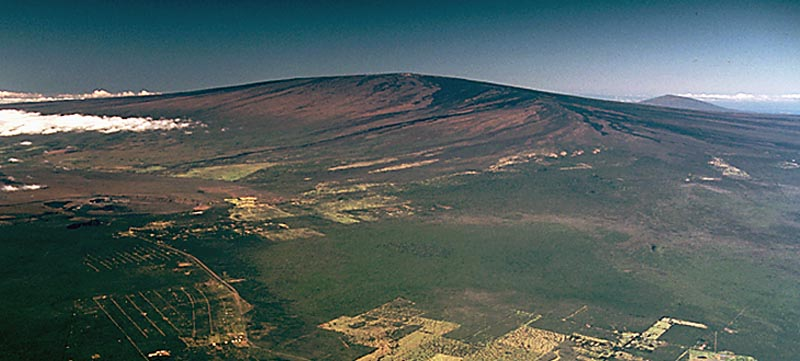
\includegraphics[width=0.8\linewidth]{images/book1/g7-mauna-loa.jpg}

{\small El Mauna Loa, un \omterm{def:g4:volcanoes-earthquakes-first-look:volcano}{volcán} en escudo de la Isla Grande de Hawái, visto
desde el aire: una \omterm{def:g1:landscapes-around-us:landform}{montaña} enorme de laderas suaves, construida por miles de
coladas de \omterm{def:g4:volcanoes-earthquakes-first-look:eruption}{lava} fluida. Fotografía: J.~D. Griggs, U.S. Geological Survey,
1985 (dominio público, vía Wikimedia Commons).}
% ledger: commons:mauna-loa
\label{fig:g7:volcanoes:mauna-loa}
\end{omfigure}

\section{Vivir con los volcanes}

Mucha gente vive cerca de los \omterm{def:g4:volcanoes-earthquakes-first-look:volcano}{volcanes}: en 1991 vivían unos 3~millones de
personas en la región que rodea el Pinatubo. Por suerte, una gran \omterm{def:g4:volcanoes-earthquakes-first-look:eruption}{erupción}
suele dar señales de aviso. El \omterm{def:g7:volcanoes:magma}{magma} que sube aparta las \omterm{def:g3:stones-pebbles-sand:rock}{rocas}: el suelo se
agrieta y tiembla con pequeños \omterm{def:g4:volcanoes-earthquakes-first-look:earthquake}{terremotos}, las laderas se hinchan, se
escapa gas. En el monte Santa Helena, los primeros pequeños \omterm{def:g4:volcanoes-earthquakes-first-look:earthquake}{terremotos}
llegaron el 16~de marzo de 1980; el 17~de mayo ya había habido más de
10\,000, y la ladera norte se había hinchado hacia fuera al menos
\qty{137}{m}. Los científicos lo midieron todo y se cerró la zona; aun así,
57~personas murieron el 18~de mayo.
% ledger: usgs:msh-lead-up, usgs:msh-flows

En el Pinatubo, en 1991, los científicos que vigilaban los \omterm{def:g4:volcanoes-earthquakes-first-look:earthquake}{terremotos}, los
gases y la hinchazón del \omterm{def:g4:volcanoes-earthquakes-first-look:volcano}{volcán} dieron el aviso a tiempo: la gente que vivía
cerca del \omterm{def:g4:volcanoes-earthquakes-first-look:volcano}{volcán} se marchó, y se salvaron al menos 5\,000 vidas.
% ledger: usgs:pinatubo-1991 (central Luzon home to about 3 million people)

\begin{remark}[No te acerques nunca a un volcán en erupción]\label{rem:g7:volcanoes:safety}
Mirar una \omterm{def:g4:volcanoes-earthquakes-first-look:eruption}{erupción} solo se puede hacer en los lugares que las autoridades
han abierto al público. Los gases, la caída de \omterm{def:g3:stones-pebbles-sand:rock}{rocas}, la costra de \omterm{def:g4:volcanoes-earthquakes-first-look:eruption}{lava}
reciente que se rompe bajo los pies y los \omterm{def:g7:volcanoes:pyroclastic-flow}{flujos piroclásticos} pueden
matar, a menudo sin aviso. Los observatorios vulcanológicos publican qué se
puede visitar sin peligro: haz siempre lo que dicen.
\end{remark}

\section{Ejercicios}

\begin{exercise}[$\star$]\label{exo:g7:volcanoes:1}
Une cada palabra con su significado: \omterm{def:g7:volcanoes:magma}{magma}; \omterm{def:g4:volcanoes-earthquakes-first-look:eruption}{lava}; \omterm{def:g7:volcanoes:magma-chamber}{cámara magmática}; \omterm{def:g7:volcanoes:vent}{boca
eruptiva}; \omterm{def:g7:volcanoes:vent}{cráter}. (a) Una depresión en forma de cuenco en lo alto de un
\omterm{def:g4:volcanoes-earthquakes-first-look:volcano}{volcán}. (b) La \omterm{def:g3:stones-pebbles-sand:rock}{roca} fundida que está bajo tierra. (c) Una abertura por la
que sale el \omterm{def:g7:volcanoes:magma}{magma}. (d) La \omterm{def:g3:stones-pebbles-sand:rock}{roca} fundida que ha salido a la superficie.
(e) Una gran bolsa de \omterm{def:g7:volcanoes:magma}{magma} a unos pocos kilómetros bajo un \omterm{def:g4:volcanoes-earthquakes-first-look:volcano}{volcán}.
\end{exercise}

\begin{exercise}[$\star$]\label{exo:g7:volcanoes:2}
¿Efusiva o explosiva? (a) \omterm{def:g1:landscapes-around-us:water}{Ríos} de \omterm{def:g4:volcanoes-earthquakes-first-look:eruption}{lava} incandescente bajan por una ladera
suave. (b) Una columna de ceniza sube \qty{35}{km} hacia el cielo. (c) Una
fuente de gotas incandescentes salta de una grieta. (d) Una avalancha de
ceniza y gas calientes baja a toda velocidad por un \omterm{def:g1:landscapes-around-us:landform}{valle}.
\end{exercise}

\begin{exercise}[$\star$]\label{exo:g7:volcanoes:3}
¿Verdadero o falso? Corrige las falsas. (a) El \omterm{def:g7:volcanoes:magma}{magma} y la \omterm{def:g4:volcanoes-earthquakes-first-look:eruption}{lava} son dos
nombres de la misma \omterm{def:g3:stones-pebbles-sand:rock}{roca} fundida, bajo tierra y en la superficie. (b) El
gas volcánico más abundante es el dióxido de carbono. (c) Un \omterm{def:g7:volcanoes:pyroclastic-flow}{flujo
piroclástico} es un \omterm{def:g1:landscapes-around-us:water}{río} de \omterm{def:g4:volcanoes-earthquakes-first-look:eruption}{lava} líquida. (d) Los \omterm{def:g4:volcanoes-earthquakes-first-look:volcano}{volcanes} de Hawái están en
un \omterm{def:g7:plate-tectonics:plate-boundary}{límite de placas}.
\end{exercise}

\begin{exercise}[$\star$]\label{exo:g7:volcanoes:4}
Usa la tabla de los colores del brillo. (a) Una \omterm{def:g4:volcanoes-earthquakes-first-look:eruption}{lava} brilla en amarillo:
di su temperatura. (b) Una colada que se está endureciendo brilla en rojo
oscuro: di su temperatura. (c) Una fotografía muestra \omterm{def:g4:volcanoes-earthquakes-first-look:eruption}{lava} naranja en el
frente de una colada y \omterm{def:g4:volcanoes-earthquakes-first-look:eruption}{lava} amarilla cerca de la \omterm{def:g7:volcanoes:vent}{boca}. ¿Dónde está más
caliente? ¿Por qué?
\end{exercise}

\begin{exercise}[$\star\star$]\label{exo:g7:volcanoes:5}
Usa el diagrama de barras de los 1\,214 \omterm{def:g4:volcanoes-earthquakes-first-look:volcano}{volcanes}. (a) ¿Cuántos \omterm{def:g4:volcanoes-earthquakes-first-look:volcano}{volcanes}
están en un \omterm{def:g7:plate-tectonics:plate-boundary}{límite de placas} (donde las \omterm{def:g7:plate-tectonics:plate}{placas} se separan, o donde una se
hunde bajo otra)? (b) ¿Qué porcentaje de todos los \omterm{def:g4:volcanoes-earthquakes-first-look:volcano}{volcanes} es eso?
(c) Comprueba que los cuatro porcentajes de la proposición suman
aproximadamente el 100~\%.
\end{exercise}

\begin{exercise}[$\star\star$]\label{exo:g7:volcanoes:6}
De los 660 conos empinados (estratovolcanes) de la lista, 564 están donde
una \omterm{def:g7:plate-tectonics:plate}{placa} se hunde bajo otra, 62 donde las \omterm{def:g7:plate-tectonics:plate}{placas} se separan y 33 en el
interior de una \omterm{def:g7:plate-tectonics:plate}{placa}. (a) Halla el porcentaje de conos empinados que están
donde una \omterm{def:g7:plate-tectonics:plate}{placa} se hunde bajo otra. (b) ¿Cuántos conos empinados quedan
para la situación ``desconocida''? (c) Usa las cuatro pistas: ¿qué clase de
\omterm{def:g4:volcanoes-earthquakes-first-look:eruption}{erupciones} cabe esperar a lo largo del Anillo de Fuego?
\end{exercise}

\begin{exercise}[$\star\star$]\label{exo:g7:volcanoes:7}
En el Kilauea, la \omterm{def:g4:volcanoes-earthquakes-first-look:eruption}{lava} sale de la \omterm{def:g7:volcanoes:vent}{boca} a unos \qty{1170}{\degreeCelsius}.
Por un túnel de \omterm{def:g4:volcanoes-earthquakes-first-look:eruption}{lava} llegó al \omterm{def:g2:water-on-earth:ocean}{mar}, a \qty{10}{km}, a unos
\qty{1140}{\degreeCelsius}. (a) ¿Cuántos grados se enfrió? (b) ¿Cuántos
grados son por kilómetro? (c) La \omterm{def:g4:volcanoes-earthquakes-first-look:eruption}{lava} al aire libre se enfría en su
superficie cientos de grados por segundo. Explica por qué la \omterm{def:g4:volcanoes-earthquakes-first-look:eruption}{lava} del túnel
se mantuvo tan caliente.
\end{exercise}

\begin{exercise}[$\star\star$]\label{exo:g7:volcanoes:8}
Las \omterm{def:g3:stones-pebbles-sand:rock}{rocas} más antiguas de Kauai tienen unos 5.5~millones de años; las de la
Isla Grande, menos de 0.7~millones de años. (a) ¿Qué isla es más antigua?
¿Por al menos cuántos millones de años? (b) ¿Qué isla está más desgastada?
¿Por qué? (c) ¿Qué isla está hoy sobre el \omterm{def:g7:volcanoes:hotspot}{punto caliente}? (d) Kauai está
al noroeste de la Isla Grande. ¿En qué dirección se lleva las islas la
\omterm{def:g7:plate-tectonics:plate}{placa} del Pacífico?
\end{exercise}

\begin{exercise}[$\star\star$]\label{exo:g7:volcanoes:9}
Las islas de Hawái están a más de \qty{3200}{km} del \omterm{def:g7:plate-tectonics:plate-boundary}{límite de placas} más
cercano. (a) ¿Por qué es sorprendente para unos \omterm{def:g4:volcanoes-earthquakes-first-look:volcano}{volcanes}? (b) Explica en
tres o cuatro frases de dónde viene su \omterm{def:g7:volcanoes:magma}{magma}. (c) En el \omterm{def:g2:drawing-to-map:map}{mapa} de los
\omterm{def:g4:volcanoes-earthquakes-first-look:volcano}{volcanes}, ¿de qué color son?
\end{exercise}

\begin{exercise}[$\star\star$]\label{exo:g7:volcanoes:10}
En junio de~1991, el primer \omterm{def:g7:volcanoes:magma}{magma} del Pinatubo salió tranquilamente; tres
días después, otro \omterm{def:g7:volcanoes:magma}{magma} explotó. Usa las dos botellas de agua con gas para
explicar la diferencia. ¿Cuál de los dos \omterm{def:g7:volcanoes:magma}{magmas} había perdido su gas al
subir?
\end{exercise}

\begin{exercise}[$\star\star\star$]\label{exo:g7:volcanoes:11}
Un pueblo está \qty{10}{km} \omterm{def:g1:landscapes-around-us:landform}{valle} abajo de un \omterm{def:g4:volcanoes-earthquakes-first-look:volcano}{volcán}. (a) Un \omterm{def:g7:volcanoes:pyroclastic-flow}{flujo
piroclástico} avanza a \qty{80}{km/h}. ¿Cuántos minutos tardaría en llegar
al pueblo? (b) La misma pregunta a \qty{130}{km/h}. (c) Una familia
necesita 20~minutos para marcharse en coche. Explica por qué el aviso tiene
que llegar antes de que empiece la \omterm{def:g4:volcanoes-earthquakes-first-look:eruption}{erupción}, y no cuando se ve el flujo.
\end{exercise}

\begin{exercise}[$\star\star\star$]\label{exo:g7:volcanoes:12}
La ceniza del monte Santa Helena dio una vuelta entera a la Tierra en
15~días. Un grado de \omterm{def:g6:latitude-longitude:latitude}{latitud} mide unos \qty{111}{km}, y una vuelta completa
son 360~grados. (a) ¿Cuánto mide, más o menos, una vuelta completa a la
Tierra, en kilómetros? Redondea al millar más cercano. (b) ¿Cuántos
kilómetros recorrió la ceniza al día, de media? (c) ¿Cuántos kilómetros por
hora son? (d) ¿Lleva la ceniza el viento o se mueve por su propia
velocidad? Explícalo.
% ledger: usgs:msh-may18, rmg:latitude-def
\end{exercise}

\section{Problema: el día en que la montaña perdió la cima}

\begin{problem}[{Problema de fin de semana --- las señales de aviso del
monte Santa Helena, la erupción del 18~de mayo de 1980 y cuánto se perdió de
la montaña}]
\label{pb:g7:volcanoes:1}
% ledger: usgs:msh-heights, usgs:msh-lead-up, usgs:msh-may18, usgs:msh-flows, usgs:msh-reach, usgs:msh-dome, usgs:msh-faq-loss, data:gvp, tht:everest

El monte Santa Helena está en el noroeste de los Estados Unidos. Usa las
fotografías del principio del capítulo, el \omterm{def:g2:drawing-to-map:map}{mapa} de los \omterm{def:g4:volcanoes-earthquakes-first-look:volcano}{volcanes} y los
números de abajo, medidos por el U.S. Geological Survey.

\medskip
\noindent\textbf{Parte I --- Antes de la erupción.}
\begin{enumerate}
  \item Los primeros pequeños \omterm{def:g4:volcanoes-earthquakes-first-look:earthquake}{terremotos} llegaron el 16~de marzo de 1980; la
        gran \omterm{def:g4:volcanoes-earthquakes-first-look:eruption}{erupción}, el 18~de mayo. ¿Cuántos días pasaron entre las dos
        fechas? (Marzo tiene 31~días, y abril, 30.)
  \item El 17~de mayo ya se habían registrado más de 10\,000 \omterm{def:g4:volcanoes-earthquakes-first-look:earthquake}{terremotos},
        en los 62~días transcurridos desde el 16~de marzo. ¿Cuántos son,
        más o menos, al día, de media?
  \item La ladera norte de la \omterm{def:g1:landscapes-around-us:landform}{montaña} se hinchó hacia fuera al menos
        \qty{137}{m}. Explica por qué la hinchazón preocupaba a los
        científicos.
  \item En el \omterm{def:g2:drawing-to-map:map}{mapa} de los \omterm{def:g4:volcanoes-earthquakes-first-look:volcano}{volcanes}, el monte Santa Helena es un triángulo
        azul. ¿Qué te dice eso de su situación? ¿Qué clase de \omterm{def:g4:volcanoes-earthquakes-first-look:eruption}{erupción}
        esperas, y qué forma de \omterm{def:g4:volcanoes-earthquakes-first-look:volcano}{volcán}?
\end{enumerate}

\medskip
\noindent\textbf{Parte II --- El 18 de mayo de 1980.}\par\nopagebreak
\begin{enumerate}[resume, beginpenalty=10000]
  \item A las 8:32, un pequeño \omterm{def:g4:volcanoes-earthquakes-first-look:earthquake}{terremoto} hizo deslizarse la ladera
        hinchada. El deslizamiento avanzó a hasta \qty{240}{km/h}. ¿Cuántos
        kilómetros por minuto son?
  \item El deslizamiento dejó el \omterm{def:g7:volcanoes:magma}{magma} al descubierto, como un tapón que se
        quita de una botella agitada. Explica por qué el \omterm{def:g4:volcanoes-earthquakes-first-look:volcano}{volcán} explotó
        entonces de lado.
  \item La explosión lateral avanzó a al menos \qty{480}{km/h} y llegó a
        \qty{27}{km} del \omterm{def:g4:volcanoes-earthquakes-first-look:volcano}{volcán}. A esa velocidad, ¿cuántos minutos tardó,
        como mucho, en llegar allí?
  \item Los \omterm{def:g7:volcanoes:pyroclastic-flow}{flujos piroclásticos} avanzaron a hasta \qty{130}{km/h} y
        llegaron a \qty{8}{km} del \omterm{def:g7:volcanoes:vent}{cráter}. ¿Cuántos minutos tardaron a esa
        velocidad? Redondea al minuto más cercano.
\end{enumerate}

\medskip
\noindent\textbf{Parte III --- Después.}\par\nopagebreak
\begin{enumerate}[resume, beginpenalty=10000]
  \item La columna de ceniza alcanzó una altura de unos \qty{24}{km} en
        menos de 15~minutos. ¿Cuántas veces más alta que el Everest
        (\qty{8.8}{km}) es? Redondea a un decimal.
  \item Entre 1980 y 1986, una \omterm{def:g4:volcanoes-earthquakes-first-look:eruption}{lava} viscosa salió lentamente en el \omterm{def:g7:volcanoes:vent}{cráter} y
        construyó un domo de \qty{267}{m} de altura sobre la \omterm{def:g7:volcanoes:vent}{boca}. ¿Fueron
        estas \omterm{def:g7:volcanoes:eruption-types}{erupciones efusivas} o explosivas? ¿Qué botella de agua con gas
        te recuerdan?
  \item Mira las dos fotografías del \omterm{def:g4:volcanoes-earthquakes-first-look:volcano}{volcán}. Describe en dos frases lo que
        cambió.
  \item Antes de la \omterm{def:g4:volcanoes-earthquakes-first-look:eruption}{erupción}, la cima estaba a \qty{2950}{m} sobre el \omterm{def:g4:world-physical-map:altitude}{nivel
        del mar}; después, el punto más alto estaba a \qty{2549}{m}. ¿Cuántos
        metros de altura perdió la \omterm{def:g1:landscapes-around-us:landform}{montaña}?
\end{enumerate}
\end{problem}
